%! Author = adam
%! Date = 28.02.21


\chapter{Beam Parameters}\label{ch:beam-parameters}

Once we have a focused beam of ions hurtling themselves at high energies towards a sample, there are a few parameters that are of particular use in both the description of the beam, and the predicting of effects of the beam.
Below is a list of parameters, and those that we will cover in closer detail are listed in \textbf{bold}.
\begin{myitemize}
	\item DC or AC
	\item Ion Type
	\item Ion Energy
	\item Charge State
	\item \textbf{Divergence, Brightness (Brilliance), Emittance}
	\item Beam Diameter
	\item \textbf{Focus Size}
	\item Working Distance
	\item \textbf{Beam Current }
	\item \textbf{Beam Shape}
	\item Beam Stability
\end{myitemize}
For example, AC or DC is a question we have already discussed in CHAPTER ION ACCELERATORS, in which beams could be a constant supply (DC), or are pulsed (AC).
In the chapter on ion sources we discussed how one would produce different ions, hence the ion types.
Ion energy is also discussed in \ref{ch:ion-sources}, but it also depends on the charge state of the ion.
The lowest beam diameter we can achieve is known as the focus size.
The beam current being the density of ions traveling towards a sample, which one may want high or low current depending on application, e.g., you want to introduce single ions into a sample, so you want very low current so that a singular ion impact is possible.

\section{Emittance and Brilliance}
In order to best understand these concepts we must revisit our lectures on theoretical mechanics, and more specifically \textit{Liouville's Theorem} and phase space.
The goal is to describe the trajectory of particles using phase space.
Liouville's Theorem helps in this regard with the fact that a volume in phase space is constant in time iff one can describe their system using a Hamiltonian.
In ion beams we normally have phase ellipse, i.e., the phase space of the ion beam is roughly in the shape of an ellipse.
The equation for a 2D ellipse is given by\[ \gamma x^2 + 2\alpha x x^{\prime} + \beta x^{\prime 2} = \epsilon \], for which the area of this 2D ellipse is given by: \[ \int_{ellipse} dxdx^\prime = \pi \epsilon \].
In both of these equations, we are in phase space, so $x$ is the position, and $x^\prime$ would be the momentum.
The phase space distribution function would then be constant along the trajectories of the system (in our case this is the ion particle system), which leads to the density of system points in vicinity of a given system point traveling through phase space is constant with time.
In the Figure~\ref{fig:PSib} we see how the phase space is changing due to a focusing lens.
But what does the brightness and emittance have to do with all of this?

\begin{figure}
	\centering
	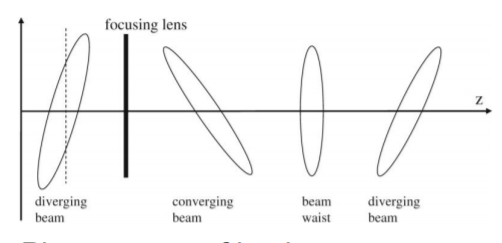
\includegraphics[width=0.7\linewidth, height = 5.5cm]{phase-space-lens}
	\caption{Via the use of a focusing lens, we see that the phase space of the diverging beam is inverted to that of the phase space of the converging beam. Then, as we reach the focal point of the beam from the use of the lens, we see that the distribution of ions has a very small width, i.e., they are centered positionally in the phase space (the focus) and the position unceratnity is low whereas there is broad uncertanity in the momentum! After the beam waist, we see the beam transforms back into a diverging beam, and we a similar phase space as we got before.  }
	\label{fig:PSib}
\end{figure}
Emittance is the measure for the average spread of particle coordinates in te phase space.
Since we clarified that the volume (or area in 2D) of the phase space stays the same over time through accelerations (lens, etc.) the position spread may change, but the emittance stays the same.
A low emittance particle beam is a beam where the particles are confined to a small distance but have nearly the same momentum.
This goes to say that a beam system will only allow particles with a particular momentum, and of course those that fit through the beam pip or magnets that make up the system.
For the geometric definition, one will see why we chose $\epsilon$ above in our definitions.
The  definition of the transverse emittance $\epsilon$ is:
\[ \epsilon = \frac{6\pi \left(width^2 - D^2 \left(\frac{dp}{p}\right)^2\right)}{B}\]
where $width$ is the width of the particle beam, $dp/p$ is the momentum spread of the beam, $D$ is the value of the dispersion function at a measurement point in the particle accelerator, $B$ is the value of the beta function at the same measurement point.
Emittance also closely related to the brightness of a beam, and can be seen in Figure~\ref{fig:bright}, where we derive equation~\ref{eq:bright}.

\begin{figure}
	\centering
	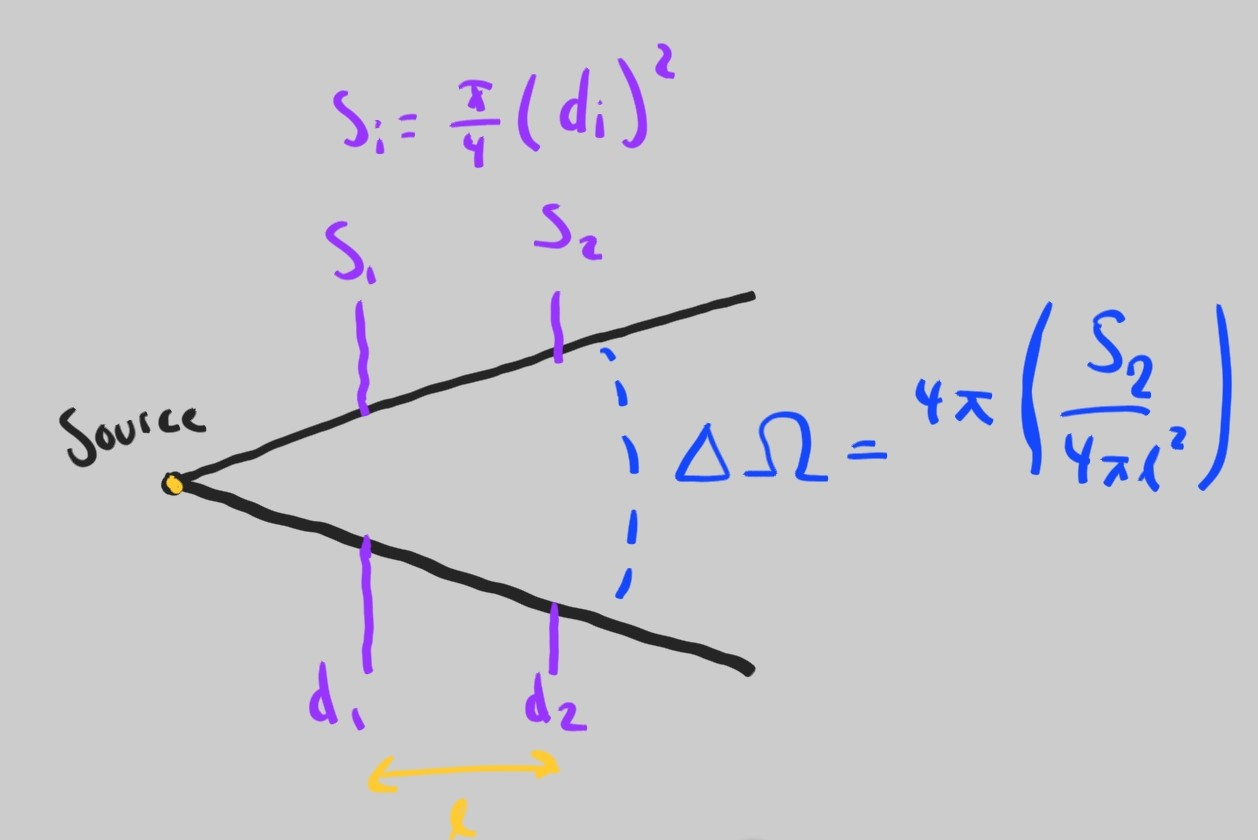
\includegraphics[width=0.5\linewidth, height=5cm]{bright}
	\caption{The ion source on the left hand side passes through two apertures $A1$ and $A2$, each aperture having a diameter denoted by $d_1$, $d_2$ and are placed a distance $l$ apart from each other. The area of the apertures is then written $S_i = \frac{\pi}{4}d_i^2$. The divergence of the beam is denoted by the solid angle $\Delta \Omega$. At the end of the second aperture we want to measure the beam current, so we place a Faraday cup grounded (the apertures are also grounded). Now the brightness is then defined $B = \frac{I}{S_1 \Delta \Omega}$. The solid angle is $\Delta \Omega = 4\pi \frac{S_2}{O}$ where  $O$ is the overall solid angle, i.e., $4\pi l^2$. This yields us finally the relationship seen in Equation \ref{eq:bright}}
	\label{fig:bright}
\end{figure}


\begin{equation}
B = \frac{I l^2}{S_1 S_2}
\label{eq:bright}
\end{equation}

There is also an equation where we normalize the brilliance w.r.t the energy of the ions $E$, which can be written:
$$ B_n = \frac{I l^2}{S_1 S_2 E} $$
For example, an ion beam with current $1.1$nA, and aperture lengths $d_1 = d_2 = 2-- \mu$m, and distance $l = 4.9$m between them, the normalize brilliance of the ion beam for ion energy $E = 2 MeV$ is $B_n = 13.5$ A/m$^2$eV.


Although emittance is normally constant, there are times when it is not.
Lens, for example, conserve it but when we use radiation damping or electron cooling, there are other effects taking place on the ions such that there can be changes in $\epsilon$


\section{Focus Size}\label{sec:focus-size}
As mentioned earlier in the chapter, the focus size is defined as the lowest possible beam diameter one can achieve.
One can focus a beam using magnetic lens just like how optical focusing works.

\section{Beam Shape}\label{sec:beam-shape}
The size of the beam is influenced by geometric demagnetization of the lens system, as well as aberration of lenses and the beam emittance.
There are many fancy ways in measuring the beam profile.
Another aspect of the beam profile is the temperature of it.
Like a collection of gas molecules, the ion beam also has a temperature.
Since particles will naturally drift apart in the accelerator (think expanding gas particles of a particular temperature), the beams must be then brought back together or else they will slam into the walls of the vacuum pipes.
But, because of this, one must think about how the ion-ion interaction is.
Let's estimate the Coulomb force between two ions.
We can estimate using a ion beam current of $I = 1$ MeV, which gives us avelocity of about 10 precent the speed of light, or $v = 3\times 10^7 $m/s.
With this current we have a number density per second of $I = \frac{Q}{t} = \frac{Ne}{t} \Rightarrow n = \frac{N}{t} \approx 6.2\times 10^5$ ions per second.
The distance per ion is then estimated $  \frac{v}{n} \approx 4.8$ mm per ion.
This finally yields us $F_C \approx 10^-23$N.
Okay it is tiny.
The Coulomb interaction can be neglected for this example, but as we said earlier, at high density, the Coulomb interaction will be much larger since the distance between ions will be much smaller!


\section{Summary}\label{sec:summary2}

\begin{itemize}
	\item Many parameters of an ion beam can be quantified, and many come from the source/acceleration.
	\item The emittance of an ion beam $\epsilon$ is held constant through the use of lenses/acceleration of particles, but can also at times not be constant due to non-linear affects (high $I \rightarrow$ high $n$ thus interactions can not be neglected) as well as radiation damping, etc.
	\item Brilliance of a beam measures the current density over an area in which the beam is focused
	\item Focus size is the lowest possible beam diameter one can achieve
	\item Beam shape is influenced by the aberration of lenses and beam emittance
	\item With low current density we can neglect the ion-ion interaction, but at higher densities we must take this into account
	\item  The measuring of a current is through the use of a faraday cup
\end{itemize}

